\documentclass[12pt,a4paper]{article}
\usepackage{lecturestyle}

\begin{document}

\section{Graphs}

\begin{definition}
A graph $G$ consists of a pair of sets $V(G)$ and $E(G)$ where $V(G)$ is a finite non-empty set of objects called \textit{vertices}, and $E(G)$ is a set of unordered pairs of vertices called \textit{edges}.
\end{definition}

\begin{example}
    Consider a graph $G$ defined by $V(G) = \{ a,b,c,d\}$ and $E(G) = \{\{a,b\}, \{b,c\}, \{b,d\}\}$ \\

    We can visualize such a graph as:\\
    
\begin{center}
\begin{minipage}{0.45\textwidth}
\centering
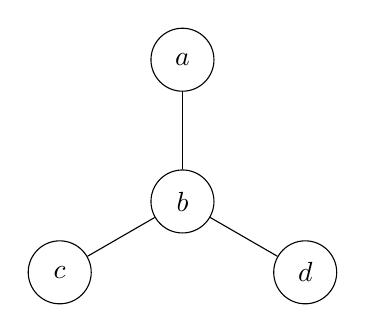
\begin{tikzpicture}[
    every node/.style={circle, draw, minimum size=8mm}
]
    \node (b) at (0,0) {$b$};
    \node (a) at (90:1.8) {$a$};
    \node (c) at (210:1.8) {$c$};
    \node (d) at (330:1.8) {$d$};

    \draw (b) -- (a);
    \draw (b) -- (c);
    \draw (b) -- (d);
\end{tikzpicture}
\end{minipage}
\hfill
\begin{minipage}{0.45\textwidth}
\centering
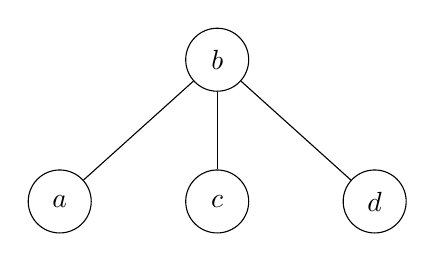
\begin{tikzpicture}[
    every node/.style={circle, draw, minimum size=8mm}
]
    \node (b) at (0,0) {$b$};
    \node (a) at (-2,-1.8) {$a$};
    \node (c) at (0,-1.8) {$c$};
    \node (d) at (2,-1.8) {$d$};

    \draw (b) -- (a);
    \draw (b) -- (c);
    \draw (b) -- (d);
\end{tikzpicture}
\end{minipage}
\end{center}

    
\end{example}


Relevant Terminology:
\begin{enumerate}
    \item $u,v$ are said to be adjacent if $\{u,v\}$ is an edge.
    \item Vertices adjacent to a fixed vertex $u$ are called neighbours of $u$. The set of all neighbours of $u$ is defined $N_G(u)$
    \item An edge $e = \{u,v\}$ is \textit{incident} with its two ends $u$ and $v$
\end{enumerate}

Course-specific information:
\begin{enumerate}
    \item $e=uv$ is used to denote the edge $e = \{u,v\}$
    \item Edges are \textit{unordered}: $uv = vu$
    \item For most of the course, we consider \textit{simple} graphs: graphs with no loops, no multiple edges:
\begin{center}
\begin{minipage}{0.45\textwidth}
\centering
\begin{tikzpicture}[
    every node/.style={
        circle, draw, minimum size=8mm,
        inner sep=0pt, outer sep=0pt
    },
    line width=0.7pt
]
    \path[use as bounding box]
        (-2,-1.1) rectangle (2,1.5);

    \node (u) at (0,0) {$u$};

    % Circular loop above the node
    \draw (u.60) arc[
        start angle=-60,
        end angle=240,
        radius=4mm
    ];
\end{tikzpicture}

\par\smallskip
Loop
\end{minipage}
\hfill
\begin{minipage}{0.45\textwidth}
\centering
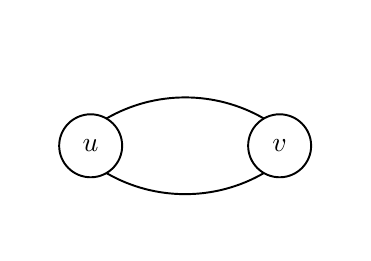
\begin{tikzpicture}[
    every node/.style={
        circle, draw, minimum size=8mm,
        inner sep=0pt, outer sep=0pt
    },
    line width=0.7pt
]
    \path[use as bounding box]
        (-2,-1.1) rectangle (2,1.5);

    \node (u) at (-1.2,0) {$u$};
    \node (v) at (1.2,0) {$v$};

    % Upper circular arc
    \draw (u.60) arc[
        start angle=120,
        end angle=60,
        radius=20mm
    ];

    % Lower circular arc
    \draw (u.-60) arc[
        start angle=240,
        end angle=300,
        radius=20mm
    ];
\end{tikzpicture}

\par\smallskip
Multiple Edges
\end{minipage}
\end{center}

    
\end{enumerate}

Graphs have many applications. Physical networks such as computer networks, electrical networks, road networks can be represented. They can be more abstract as well, such as social networks. Finally, they are also used as data structures in computer science.

\begin{definition}
    The \textit{degree} of a vertex $v$ in a graph $G$ is the number of edges incident with $v$. We write $\deg_G(v)$ or just $\deg(v)$ if $G$ is understood (in other words, $G$ has a set $V$ and $E$ representing the graph). Alternatively, $\deg(v) = \lvert N_G(v)\rvert$\\
\end{definition}

\end{document}
